\subsection*{Overview}

In order to interact with the robot aside of speech, a web-based Graphical User Interface (GUI) has been designed. An HTML5 website\footnote{\texttt{https://github.com/tue-robotics/tue\_mobile\_ui}} is hosted on the robotic platform that offers a GUI to multiple users on different platforms with use of a Robot API\footnote{\texttt{https://github.com/tue-robotics/robot-api}} implemented in Javascript. Figure~\ref{fig:webgui_architecture} shows an overview of how the user can interact with the robot via this interface.

\begin{figure}[ht]
        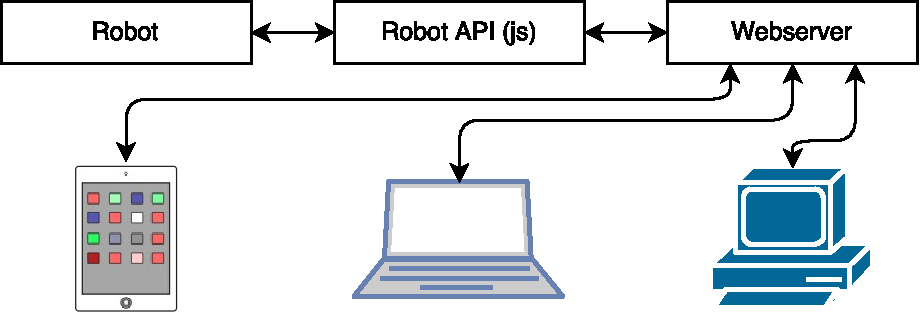
\includegraphics[width = \linewidth]{webgui_architecture}
        \caption{Overview webGUI architecture. The robot's functionalities are exposed with use of the Robot API that is implemented in javascript. The Webserver that is hosting the GUI connects this Robot API to a graphical user interface that is offered to multiple clients on different platforms.}
        \label{fig:webgui_architecture}
\end{figure}


